%###########################PRESENTACION##########################################
%Modo presentación
\documentclass[]{beamer}

%Modo handout
%\documentclass[handout,compress]{beamer}
%\usepackage{pgfpages}
%\pgfpagesuselayout{4 on 1}[border shrink=1mm]

\usepackage{graphicx}
\usepackage{beamerthemeCambridgeUS}
\usepackage{subfig}
\usepackage{tikz}
\usepackage{amsmath}
\usepackage{ragged2e}
\setbeamercovered{transparent}

\graphicspath{{G:/My Drive/FIGURAS/}}

\title[Introducción]{SENSORES REMOTOS}
\author[Edier Aristizábal]{Edier V. Aristizábal G.}
\institute{\emph{evaristizabalg@unal.edu.co}}
\date{(Versión:\today)}
\usepackage{textpos} 

\addtobeamertemplate{headline}{}{%
	\begin{textblock*}{2mm}(.9\textwidth,0cm)
	\hfill
\includegraphics[height=1cm]{un}  
	\end{textblock*}
			}
%############################INICIO#############################################
\begin{document}
%###########################SLIDE
\begin{frame}
\titlepage
\centering
	
\includegraphics[width=5cm]{unal}\hspace*{4.75cm}~%
   	\includegraphics[width=2cm]{logo3} 
\end{frame}
%#############################SLIDE
\begin{frame}
\frametitle{Introducción}
\justifying
\small{Curso teórico práctico (100\%) de 3 créditos académicos, lo que significa 9 horas semanales de dedicación en promedio durante todo el semestre... eso significa unas semanas menos horas y otras muchas mas horas.\vfill
\par La información del curso, tales como programa, presentaciones, lecturas recomendadas, talleres y demás podrá ser consultado en \emph{Google Classroom}:\vfill

\url{https://classroom.google.com}\vfill


\par Por favor visiten esta página y el programa. Allí pueden encontrar el programa con todas las fechas e información del curso.\vfill

\par Este  a no  el  curso  se  enfoca  en  herramientas  digitales  y  no  se  realizará  salida  de campo.
}
\end{frame}
%#############################SLIDE
\begin{frame}
\frametitle{Curso: Sensores Remotos}
\justifying
\small{
La información del curso, tales como programa, lecturas recomendadas y demás podrá ser consultado en Classroom:\vfill
\begin{center}
\url{https://classroom.google.com/u/0/c/NjI1NzExOTU0MTFa}\\
Class code: [coi7txj]\\
\includegraphics[width=10cm]{classroom_SR}
\end{center}}
\end{frame}
%#############################SLIDE
\begin{frame}
\frametitle{Objetivos y alcance del curso}
\justifying
\small{
\par El curso de Sensores Remotos está orientado para estudiantes de ciencias de la tierra con el objeto de aprender a utilizar las herramientas de teledetección en geología y geomorfología. Inicialmente comprende la teoría general de sensores remotos y procesamiento de imágenes. Para posteriormente enfocarse en el uso de fotografías aéreas y adquirir de forma adecuada la técnica de la fotointerpretación a través del uso de fotografías aéreas.\vfill
\par Este curso no corresponde a un curso a profundidad y detalle del uso de imágenes de satélite para diferentes disciplinas. De forma similar, la técnica de fotointerpretación, aunque es similar para otros temas, su aplicación en este curso se enfoca exclusivamente para la fotointerpretación geológica, es decir diferenciar unidades litológicas, al igual que fotointerpretación geomorfológica, es decir formas y procesos morfodinámicos.\vfill
\par El procesamiento de imágenes es una herramienta ampliamente utilizada actualmente, y la fotointerpretación es una técnica que se conserva por su ayuda en diferentes campos, y que no puede suplir ningún otro sensor remoto. Adquirir estas herramientas seguramente le ampliará sus perspectivas profesionales en el campo de la geología aplicada a la ingeniería.
}
\end{frame}
%#############################SLIDE
\begin{frame}
\frametitle{Recomendación}
\justifying
\small{
Para tomar el curso se recomienda al estudiante haber realizado su núcleo básico y los cursos SIG, Campo I, Geomorfología, Rocas Sedimentarias, Rocas Metamórficas, Rocas Ígneas, y Geología Estructural. De esta forma el estudiante podrá sacar el máximo beneficio del contenido del curso.\vfill 

En caso que el estudiante no haya cursado las anteriores asignaturas se recomienda que cancele el curso…o este dispuesto a trabajar mucho mas duro que el resto de sus compañeros.\vfill

En cualquier caso se recomienda que revise su carga académica para este semestre, y tome una decisión responsable si tiene el tiempo suficiente para dedicarle a este curso. Seguramente otro año lo podrá tomar. Por que en caso contrario tiene alta posibilidades de perder el curso. \vfill
\begin{center}
\textbf{Este curso es muy fácil de ganar…pero hay que trabajar mucho.}
\end{center}
}
\end{frame}
%#############################SLIDE
\begin{frame}
\frametitle{Definición}
\justifying
\small{
Los Sensores Remotos (teledetección) es el \textbf{arte, ciencia y tecnología} de observar un \textbf{objeto, escena o fenómeno} por técnicas basadas en instrumentos. El termino “remoto” se refiere a la observación realizada a una distancia \textbf{sin contacto físico} con el objeto de interés. Se puede utilizar herramientas de detección y despliegue en tiempo real o una herramienta que registra la \textbf{energía}, la cual es \textbf{emitida o reflejada} desde el objeto o la escena en observación. La energía puede ser luz u otra forma de radiaciones electromagnética, campos de fuerza o energía acústica.\vfill
\begin{center}
\includegraphics[width=6cm]{sensoresremotos}
\end{center}}
\end{frame}
%#############################SLIDE
\begin{frame}
\frametitle{Sensores Remotos}
\begin{center}
\includegraphics[width=11cm]{sensoresremotos1}
\end{center}
\end{frame}
%#############################SLIDE
\begin{frame}
\frametitle{Sensores Remotos}
\begin{center}
\includegraphics[width=11cm]{sensoresremotos2}
\end{center}
\end{frame}
%#############################SLIDE
\begin{frame}
\frametitle{Sensores Remotos}
\begin{center}
\includegraphics[width=12cm]{sensoresremotos3}
\end{center}
\end{frame}
%#############################SLIDE
\begin{frame}
\frametitle{Historia (I)}
\framesubtitle{Antes de 1900}
\begin{columns}
\begin{column}{0.5\textwidth}
\begin{itemize}
\item Invento de la fotografía en \textbf{1829} Nicephore Niepce, William Henry Fox Talbot, Louis Jacques Mande Daguerre
\item Invento del estereoscopio en \textbf{1839} por  Charles Wheatstone
\item Primera F. aérea en \textbf{1858} sobre Paris (Val de Bievre) desde aprox. 400 m en globo (Gaspard-felix Tournachon \emph{Nadar})
\end{itemize}
\end{column}
\begin{column}{0.5\textwidth}
\begin{center}
\includegraphics[width=5cm]{nadar}
\end{center}
\end{column}
\end{columns}
\end{frame}
%#############################SLIDE
\begin{frame}
\frametitle{Primera fotografia}
\begin{center}
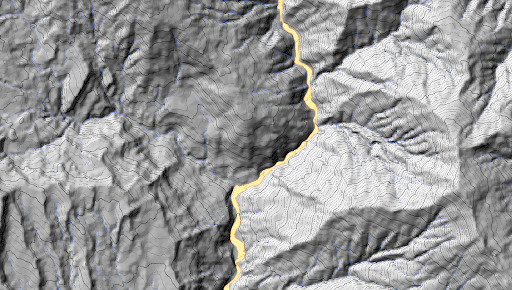
\includegraphics[width=11cm]{foto1}
\end{center}
\end{frame}
%#############################SLIDE
\begin{frame}
\frametitle{Primera fotografia aérea desde globo (Boston -1860)}
\begin{center}
\includegraphics[width=5.7cm]{boston}
\end{center}
\end{frame}
%#############################SLIDE
\begin{frame}
\frametitle{San Francisco (1906) - 6 semanas despues del terremoto}
\begin{center}
\includegraphics[width=12cm]{sanfrancisco}
\end{center}
\end{frame}
%#############################SLIDE
\begin{frame}
\frametitle{Historia (II)}
\framesubtitle{Entre 1900-1950}
\small{
\begin{itemize}
\item 1909 $\rightarrow$ Wibur Wright adquiere la primera fotografía aérea sobre Le Mans (Francia).
\item 1915 $\rightarrow$ Lt. Col. J.T.C. Brabazon diseñaron y produjeron la primera cámara aérea.
\item 1919 $\rightarrow$ Inicia el Programa Canadiense para el mapeo de bosques. 
\item 1940 $\rightarrow$ La WW I \& WW II trajo consigo el desarrollo de técnicas mas sofisticadas de fotointerpretación.
\end{itemize}
}
\begin{center}
\includegraphics[width=10cm]{fotoaerea_ww}
\end{center}
\end{frame}
%#############################SLIDE
\begin{frame}
\frametitle{Historia (III)}
\framesubtitle{Despues de 1950}
\small{
\begin{itemize}
\item 1946 $\rightarrow$ Primera fotografía desde el espacio V-2 rockets.
\item 1960 $\rightarrow$ Es lanzado el primer satélite meteorológico TIROS-1.
\item 1960 $\rightarrow$ Estados unidos da inicio al programa de fotografías para inteligencia desde satélites CORONA.
\item 1972 $\rightarrow$ Es lanzado el ERTS-1, el primer satélite para estudiar los recurso de la tierra (Earth Resources Technology Satellite, mas tarde renombrado Landsat 1).  
\end{itemize}
}
\begin{center}
\includegraphics[width=4cm]{tiros1_1}
\end{center}
\end{frame}
%#############################SLIDE
\begin{frame}
\begin{center}
\includegraphics[width=8.5cm]{v2rockets}
\end{center}
\end{frame}
%#############################SLIDE
\begin{frame}
\begin{center}
\includegraphics[width=7.7cm]{tiros1}
\end{center}
\end{frame}
%#############################SLIDE
\begin{frame}
\frametitle{Actualidad}
\begin{center}
\includegraphics[width=10cm]{remotesensing_all}
\end{center}
\end{frame}
%#############################SLIDE
\begin{frame}
\frametitle{Actualidad}
\begin{center}
\includegraphics[width=10cm]{remotesensing_all1}
\end{center}
\end{frame}
%#############################SLIDE
\begin{frame}
\frametitle{Aplicaciones}
\begin{center}
\includegraphics[width=10cm]{remotesensing_usos}
\end{center}
\end{frame}
%#############################SLIDE
\end{document}